\documentclass[12pt,a4paper]{article}

\title{Super concrete computations of the cohomology ring of the torus}
\author{Benjamin Thompson}
\date{November 22, 2020}

\usepackage{tikz}
\usetikzlibrary{decorations.markings}

\usepackage{amsmath}

\newcommand{\Oplus}{\bigoplus}

\newcommand{\Ext}{\text{Ext}}
\newcommand{\Hom}{\text{Hom}}

\newtheorem{theorem}{Theorem}
\newtheorem{defin}{Definition}

\begin{document}
\maketitle

Cohomology is everywhere in modern mathematics, yet many people learning it for the first time find it scary. The confusion can come from the mass of technical homological algebra which surrounds the topological concepts. While the algebra provides a framework necessary to prove general results, it can obfuscate what actually happens in simple cases.
\[
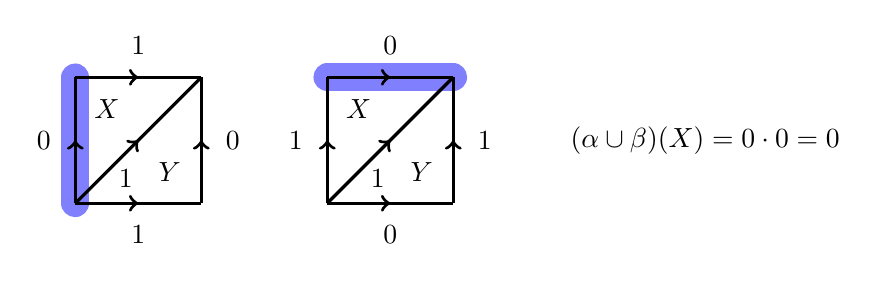
\begin{tikzpicture}[auto,semithick, scale=0.8]
  % a _ b (X)
  \begin{scope}[scale=1,xshift=0cm,very thick]
    \draw[white!50!blue, line width=10pt, line cap=round] (0,0) -- (0,2);
    \begin{scope}[decoration={markings, mark=at position 0.5 with {\arrow{>}}}]
      \draw[postaction={decorate}] (0,0) -- (0,2);
      \draw[postaction={decorate}] (0,0) -- (2,0);
      \draw[postaction={decorate}] (0,2) -- (2,2);
      \draw[postaction={decorate}] (2,0) -- (2,2);
      \draw[postaction={decorate}] (0,0) -- (2,2);
    \end{scope}
    \node (a1) at (1,-0.5)  {$1$};
    \node (a2) at (1,2.5)   {$1$};
    \node (b1) at (-0.5,1)  {$0$};
    \node (b2) at (2.5,1)   {$0$};
    \node (c)  at (0.8,0.4) {$1$};
    \node (X)  at (0.5,1.5) {$X$};
    \node (Y)  at (1.5,0.5) {$Y$};
  \end{scope}
  \begin{scope}[scale=1,xshift=4cm,very thick]
    \draw[white!50!blue, line width=10pt, line cap=round] (0,2) -- (2,2);
    \begin{scope}[decoration={markings, mark=at position 0.5 with {\arrow{>}}}]
      \draw[postaction={decorate}] (0,0) -- (0,2);
      \draw[postaction={decorate}] (0,0) -- (2,0);
      \draw[postaction={decorate}] (0,2) -- (2,2);
      \draw[postaction={decorate}] (2,0) -- (2,2);
      \draw[postaction={decorate}] (0,0) -- (2,2);
    \end{scope}
    \node (a1) at (1,-0.5)  {$0$};
    \node (a2) at (1,2.5)   {$0$};
    \node (b1) at (-0.5,1)  {$1$};
    \node (b2) at (2.5,1)   {$1$};
    \node (c)  at (0.8,0.4) {$1$};
    \node (X)  at (0.5,1.5) {$X$};
    \node (Y)  at (1.5,0.5) {$Y$};
  \end{scope}
  \node (m) at (10,1) {$(\alpha \cup \beta) (X) = 0 \cdot 0 = 0$};
\end{tikzpicture}
\]
\[
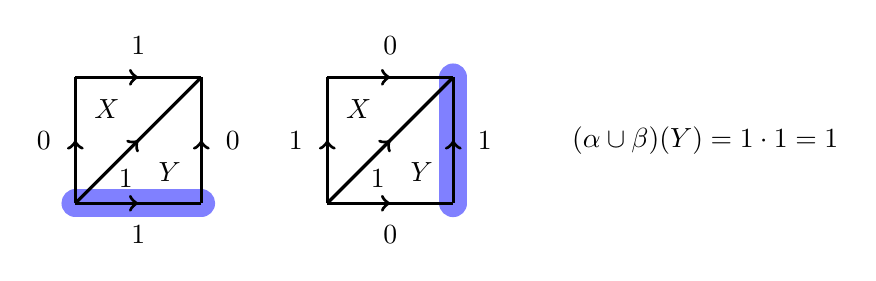
\begin{tikzpicture}[auto,semithick, scale=0.8]  
  % a _ b (Y)
  \begin{scope}[scale=1,xshift=0cm,very thick]
    \draw[white!50!blue, line width=10pt, line cap=round] (0,0) -- (2,0);
    \begin{scope}[decoration={markings, mark=at position 0.5 with {\arrow{>}}}]
      \draw[postaction={decorate}] (0,0) -- (0,2);
      \draw[postaction={decorate}] (0,0) -- (2,0);
      \draw[postaction={decorate}] (0,2) -- (2,2);
      \draw[postaction={decorate}] (2,0) -- (2,2);
      \draw[postaction={decorate}] (0,0) -- (2,2);
    \end{scope}
    \node (a1) at (1,-0.5)   {$1$};
    \node (a2) at (1,2.5)    {$1$};
    \node (b1) at (-0.5,1)   {$0$};
    \node (b2) at (2.5,1)    {$0$};
    \node (c)  at (0.8,0.4)  {$1$};
    \node (X)  at  (0.5,1.5) {$X$};
    \node (Y)  at  (1.5,0.5) {$Y$};
  \end{scope}
  \begin{scope}[scale=1,xshift=4cm,very thick]
    \draw[white!50!blue, line width=10pt, line cap=round] (2,0) -- (2,2);
    \begin{scope}[decoration={markings, mark=at position 0.5 with {\arrow{>}}}]
      \draw[postaction={decorate}] (0,0) -- (0,2);
      \draw[postaction={decorate}] (0,0) -- (2,0);
      \draw[postaction={decorate}] (0,2) -- (2,2);
      \draw[postaction={decorate}] (2,0) -- (2,2);
      \draw[postaction={decorate}] (0,0) -- (2,2);
    \end{scope}
    \node (a1) at (1,-0.5)  {$0$};
    \node (a2) at (1,2.5)   {$0$};
    \node (b1) at (-0.5,1)  {$1$};
    \node (b2) at (2.5,1)   {$1$};
    \node (c)  at (0.8,0.4) {$1$};
    \node (X)  at (0.5,1.5) {$X$};
    \node (Y)  at (1.5,0.5) {$Y$};  
  \end{scope}
  \node (m) at (10,1) {$(\alpha \cup \beta) (Y) = 1 \cdot 1 = 1$};
\end{tikzpicture}
\]

The diagrams above calculate part of the cup product structure on a torus by multiplying numbers on edges together. Multiplying 0s and 1s together is not difficult! Yet, many students encountering the cup product for the first time find it difficult to understand, and I think this is in no small part due to a lack of detailed examples.

This blog post is simply an effort to show that computing the cohomology ring of a simple space can be straightforward, by using the torus as an example. We do the calculation in two different ways. We try and keep both computations as streamlined yet self-contained as possible. 
While the following discussion may be `simple' to anyone who has studied algebraic topology for a few years, cohomology is not simple for people learning it for the first time! This note is intended for anyone who wants to see a concrete cohomology ring calculation with almost all the steps explained.

The first calculation is done in a more abstract way than the second calculation, but is quicker. The second calculation involves constructing a diagram of the torus and using the combinatorial information in it to compute the cohomology ring. Throughout we assume only that the reader has a basic understanding of abstract algebra and point-set topology. In particular, we assume the reader knows the definition of a chain complex, the homology groups of a chain complex, and a simplex.

\section*{Computing the ring structure via the K\"unneth theorem (i.e. without diagrams)}

Let us first compute the cohomology ring of the torus over the integers, denoted $H^*(T;Z)$, and do so quickly with algebra. This method is more abstract, and hence it may be harder to completely follow than the second method if the reader is still familiarizing themselves with abstract algebra.

Write the torus as a cross product of simpler spaces: $T = S^1 \times S^1$. We will be able to use this decomposition to build the cohomology ring of $T$ from the cohomology ring of $S^1$.

It is well-known that the cohomology ring of a sphere $S^k$ over the integers is the exterior algebra on one generator in degree $k$ over $Z$: $H^*(S^k;Z) \cong \Lambda_Z(a_k)$. This ring can be expressed as the quotient of a polynomial ring by an ideal:  $\Lambda_Z(a_k) \cong Z[a_k]/(a_k^2)$.

We now use the following theorem (Theorem 3.15 in Hatcher's \emph{Algebraic Topology}) to relate $H^*(S^1;Z)$ and $H^*(T;Z)$.

\begin{theorem}[K\"unneth Theorem]
  Let $X$ and $Y$ be CW complexes. 

  If the cohomology groups $H^k(Y;R)$ are finitely generated for all $k$, then there is a ring isomorphism
  \[
  H^*(X;R) \otimes_R H^*(Y;R) \overset{\cong}{\rightarrow} H^*(X \times Y ; R).
  \]
  Multiplication on the tensor product is defined by $(a \otimes b)(c \otimes d) = (-1)^{|b||c|}ac \otimes bd$, where $| f |$ denotes the degree (dimension) of $f$.
\end{theorem}

A circle is a CW complex and $\Lambda_Z(a_1)$ is finitely generated, so we can apply the theorem:
\[
H^*(T;Z) = H^*(S^1 \times S^1;Z) \cong H^*(S^1;Z) \otimes_Z H^*(S^1;Z) = \Lambda_Z(a_1) \otimes_Z \Lambda_Z(a_1).
\]
Using the definition of multiplication on this tensor product, it is easy to check that $(a_1 \otimes 1)^2 = 0 = (1 \otimes a_1)^2$, $1 \otimes 1$ is the multiplicative unit, and $(a_1 \otimes 1)(1 \otimes a_1) = a_1 \otimes a_1 = -(1 \otimes a_1)(a_1 \otimes 1)$. This leads to a graded ring isomorphism $\Lambda_Z(a_1) \otimes_Z \Lambda_Z(a_2) \cong Z[x_1,y_1]/(x_1^2,y_1^2,x_1y_1 + y_1x_1)$. This polynomial quotient is simply the exterior algebra generated by two elements, denoted $\Lambda_Z(x_1,y_1)$. Therefore $H^*(T;Z) \cong \Lambda_Z(x_1,y_1)$.

And we're done! This computation was quick, but it was quite abstract and assumed that the cohomology of $S^1$ was known. It also used the fact that the torus can be decomposed into a product of simpler spaces. Most spaces cannot be decomposed in this way, and so the method we used cannot be applied in general. Additionally, at no stage did the method give us an understanding of what the ring multiplication was geometrically.

It is possible to compute the cohomology ring of the torus without relying on this decomposition method, and also gain a geometric understanding of what the multiplication actually is. This method will take much more work, yet will involve working with a diagram of $T^2$ and so it will be more geometric.

\section*{Computing the ring structure via simplicial cohomology (i.e. with diagrams)}

There are several types of cohomology. The standard cohomology of a space is typically the singular cohomology. This type of cohomology is fairly abstract, which makes proving general results with it easier, but makes calculations harder. Simplicial cohomology is less abstract, which makes proving general results with it harder, but makes calculations easier. For sufficiently nice spaces, these two cohomology rings are actually isomorphic. The torus is an example of such a space. Therefore when we calculate the simplicial cohomology of the torus below, we also calculate its singular cohomology.

Calculating simplicial cohomology roughly involves the following steps.
\begin{enumerate}
\item Construct a simplicial diagram of the space.
\item Use this diagram to construct a chain complex and calculate cohomology groups.
\item Combine the groups together and use the diagram to calculate the ring structure.
\end{enumerate}

While these calculations could be summarized in a page (or maybe even a paragraph), we will not do so here. Instead, we will present each step of the calculation in very concrete detail so as to be more useful for people learning this content for the first time.

\subsection*{Constructing a simplicial diagram of the torus}

It can be shown using elementary point-set topology that the map $f:R \rightarrow C$ defined by $x \mapsto e^{2\pi ix}$ descends to a continuous bijection $\bar f : R / Z \rightarrow S^1$. Here $R / Z$ denotes the equivalence classes of the real numbers under $x \sim y$ when $x - y \in Z$, and is equipped with the quotient topology. Since $R/Z$ is compact and $S^1$ is Hausdorff, this map is a homeomorphism.

Similarly, it is possible to define a map to show that $R^2/Z^2$ is homeomorphic to $S^1 \times S^1 = T$. As such, we may denote the torus as the unit square with the sides identified as follows.

\[
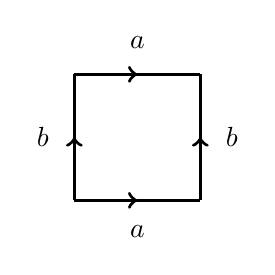
\begin{tikzpicture}[auto,semithick, scale=0.8]
  \begin{scope}[scale=1,xshift=-9cm,very thick,decoration={
        markings, mark=at position 0.5 with {\arrow{>}}}]
    \draw[postaction={decorate}] (0,0) -- (0,2);
    \draw[postaction={decorate}] (0,0) -- (2,0);
    \draw[postaction={decorate}] (0,2) -- (2,2);
    \draw[postaction={decorate}] (2,0) -- (2,2);
    
    \node (a1) at (1,-0.5) {$a$};
    \node (a2) at (1,2.5) {$a$};
    \node (b1) at (-0.5,1) {$b$};
    \node (b2) at (2.5,1) {$b$};
  \end{scope}
\end{tikzpicture}
\]

The labels and arrows indicate which edges are the same in the quotient topology. Simplicial cohomology requires us to divide up the diagram into simplices, which we can do by adding another edge.
\begin{equation}
  \label{simp-diag}
  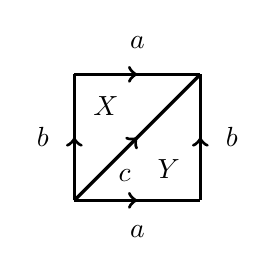
\begin{tikzpicture}[auto,semithick, scale=0.8]
    \begin{scope}[scale=1,xshift=-9cm,very thick,decoration={
          markings, mark=at position 0.5 with {\arrow{>}}}]
      \draw[postaction={decorate}] (0,0) -- (0,2);
      \draw[postaction={decorate}] (0,0) -- (2,0);
      \draw[postaction={decorate}] (0,2) -- (2,2);
      \draw[postaction={decorate}] (2,0) -- (2,2);
      \draw[postaction={decorate}] (0,0) -- (2,2);
      
      \node (a1) at (1,-0.5)  {$a$};
      \node (a2) at (1,2.5)   {$a$};
      \node (b1) at (-0.5,1)  {$b$};
      \node (b2) at (2.5,1)   {$b$};
      \node (c)  at (0.8,0.4) {$c$};

      \node (X)  at (0.5,1.5) {$X$};
      \node (Y)  at (1.5,0.5) {$Y$};
    \end{scope}
  \end{tikzpicture}
\end{equation}
The vertices of the simplices need to be ordered to compute simplicial cohomology. The arrows in the previous diagram denote which edges are the same, but we can also use them to put an ordering on the vertices of the triangles. If we require that the arrows go from smaller to larger numbers, the following is a possible ordering.
\begin{equation}
  \label{ord-diag}
  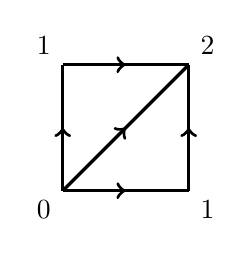
\begin{tikzpicture}[auto,semithick, scale=0.8]
    \begin{scope}[scale=1,xshift=-9cm,very thick,decoration={
          markings, mark=at position 0.5 with {\arrow{>}}}]
      \draw[postaction={decorate}] (0,0) -- (0,2);
      \draw[postaction={decorate}] (0,0) -- (2,0);
      \draw[postaction={decorate}] (0,2) -- (2,2);
      \draw[postaction={decorate}] (2,0) -- (2,2);
      \draw[postaction={decorate}] (0,0) -- (2,2);
      
      \node (00) at (-0.3,-0.3) {$0$};
      \node (01) at (-0.3,2.3)  {$1$};
      \node (10) at (2.3,-0.3)  {$1$};
      \node (11) at (2.3,2.3)   {$2$};
    \end{scope}
  \end{tikzpicture}
\end{equation}

\subsection*{Constructing the chain complex and calculating the cohomology groups}

We now use the diagrams above to construct a simplicial chain complex, calculate a cochain complex, and then calculate the homology groups of the cochain complex. The result of these steps will be the cohomology groups of the torus.

The simplicial chain groups $C_n(T)$ are free abelian groups generated by the $n$-simplices. The labels in Diagram~\ref{simp-diag} above therefore give us the chain groups:
\[
0 \rightarrow Z\{X\} \oplus Z\{Y\} \xrightarrow{\partial_2} Z\{a\} \oplus Z\{ b \} \oplus Z \{c\} \xrightarrow{\partial_1} Z\{*\} \rightarrow 0.
\]
Here $*$ denotes the common endpoint of all of the edges. The differentials $\partial_n$ of this complex require a bit of calculation, although this is purely combinatorial.

Given a $n$-simplex $\sigma : \Delta^n \rightarrow X$ and a subset $S \subset \{ 0, 1, \ldots, n \}$, define $\sigma_S$ to be the restriction of $\sigma$ to the simplex formed after removing the defining vertices of $\sigma$ corresponding to $S$. (Create it by taking the convex hull of the remaining points.) For example, for a $1$-simplex $\sigma : [0,1] \rightarrow X$, $\sigma_{\{1\}} = \sigma_{|0}$. To simplify notation for the rest of this blog, if $S$ consists only of a single element $i$, we will write $\sigma_i$ instead of $\sigma_{\{i\}}$.

The differentials $\partial_n:C_n(X) \rightarrow C_{n-1}(X)$ between simplicial chain groups are defined on $n$-simplices $\sigma : \Delta^n \rightarrow X$ by
\begin{equation}
  \label{diff-def}
  \partial_n (\sigma) := \sum_{i = 0}^n (-1)^n \sigma_{i}.
\end{equation}
Define $\partial_n$ on the chain groups by extending these maps linearly.

For example, let $\sigma : [0,1] \rightarrow X$ by a $1$-simplex. Then $\partial_1(\sigma) = \sigma_{|1} - \sigma_{|0}$. In our simplicial diagram for $T$ in Diagram~\ref{simp-diag}, all of the $1$-simplices have the same endpoints, so $\partial_1(a) = \partial_1(b) = \partial_1(c) = 0$. Since $C_1(T)$ is generated by $a,b,c$, this means that $\partial_1 = 0$.

To evaluate $\partial_2$, we need to calculate what $\partial_2$ is on the generators of $C_2(T)$, which are $\{ X,Y \}$. Note from Diagrams~\ref{simp-diag} and \ref{ord-diag} that $X_{0} = a$, $X_{1} = c$, $X_2 = b$, and $Y_0 = b$, $Y_1 = c$, $Y_2 = a$. So from equation (\ref{diff-def}) we get $\partial_2(X) = a - c + b$, and $\partial_2(Y) = b - c + a$. Note that $\partial_2(X) = \partial_2(Y)$.

We have finished calculating all of the nontrivial differentials $\partial_i$, so the simplicial chain complex is therefore isomorphic to
\[
0 \rightarrow Z^2 \xrightarrow{\left(\begin{smallmatrix}
    1 & 1 \\
    1 & 1 \\
    -1 & -1 
  \end{smallmatrix}\right)} Z^3 \xrightarrow{0} Z \rightarrow 0.
\]
If we were interested in calculating the homology groups of the torus, all we would need to do is calculate the homology of this chain complex. We are interested in the cohomology though, so we need to calculate the homology groups of the \emph{cochain} complex.

We obtain the cochain complex by applying the $\Hom(-,Z)$ functor to the groups and the maps. The canonical isomorphisms $\Hom(Z,Z) \cong Z$ and $\Hom(A \oplus B,Z) \cong \Hom(A,Z) \oplus \Hom(B,Z)$ combine to give $\Hom(Z^n,Z) \cong Z^n$. So in our case applying $\Hom(-,Z)$ to the chain groups did not change them up to isomorphism.

Applying the $\Hom(-,Z)$ functor to the differentials involves taking their dual. It is a simple exercise to show that for a linear transformation $A:Z^a \rightarrow Z^b$, the dual $A^* : Z^b \rightarrow Z^a$ is given by the adjoint matrix $A^T$.

Therefore our cochain simplicial complex is
\[
0 \leftarrow Z^2 \xleftarrow{\left(\begin{smallmatrix}
    1 & 1 & -1 \\                               
    1 & 1 & -1                          
  \end{smallmatrix}\right)} Z^3 \xleftarrow{0} Z \leftarrow 0.
\]
Now we need to calculate the homology groups of it.

The maps going into and out of the $0$th cochain group are both $0$, therefore $H^0(T;Z) \cong Z$. The map going into the $1$st cochain group is $0$, so $H^1(T;Z)$ will be isomorphic to the kernel of the matrix.

It is easy to see that the kernel of $\left(\begin{smallmatrix}
  1 & 1 & -1 \\
  1 & 1 & -1
\end{smallmatrix}\right)$ is generated by $\{ (1,0,1),(0,1,1) \}$. Recalling that $Z^3 \cong \Hom(Z^3,Z)$, these elements in the kernel are really the maps $\{ a \mapsto 1, \; b \mapsto 0, \; c \mapsto 1 \}$ and $\{ a \mapsto 0, \; b \mapsto 1, \; c \mapsto 1 \}$.

It will be useful for the cup product calculations later to denote these maps on the simplicial diagrams.

\begin{equation}
  \label{anno-diag}
  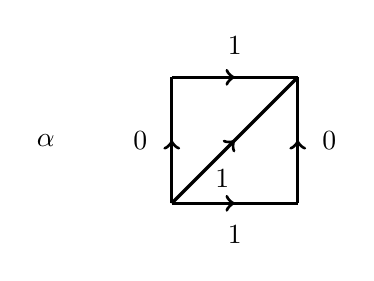
\begin{tikzpicture}[auto,semithick, scale=0.8]
    \begin{scope}[scale=1,xshift=-9cm,very thick,decoration={
          markings, mark=at position 0.5 with {\arrow{>}}}]
      \draw[postaction={decorate}] (0,0) -- (0,2);
      \draw[postaction={decorate}] (0,0) -- (2,0);
      \draw[postaction={decorate}] (0,2) -- (2,2);
      \draw[postaction={decorate}] (2,0) -- (2,2);
      \draw[postaction={decorate}] (0,0) -- (2,2);
      
      \node (a1) at (1,-0.5)  {$1$};
      \node (a2) at (1,2.5)   {$1$};
      \node (b1) at (-0.5,1)  {$0$};
      \node (b2) at (2.5,1)   {$0$};
      \node (c)  at (0.8,0.4) {$1$};

      \node (a)  at (-2,1)    {$\alpha$};
    \end{scope}
  \end{tikzpicture}
  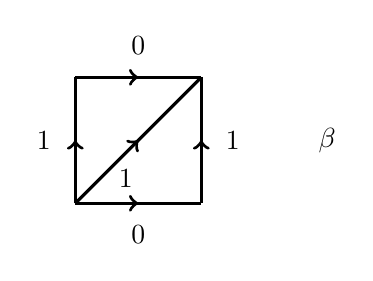
\begin{tikzpicture}[auto,semithick, scale=0.8]
    \begin{scope}[scale=1,xshift=-9cm,very thick,decoration={
          markings, mark=at position 0.5 with {\arrow{>}}}]
      \draw[postaction={decorate}] (0,0) -- (0,2);
      \draw[postaction={decorate}] (0,0) -- (2,0);
      \draw[postaction={decorate}] (0,2) -- (2,2);
      \draw[postaction={decorate}] (2,0) -- (2,2);
      \draw[postaction={decorate}] (0,0) -- (2,2);
      
      \node (a1) at (1,-0.5)  {$0$};
      \node (a2) at (1,2.5)   {$0$};
      \node (b1) at (-0.5,1)  {$1$};
      \node (b2) at (2.5,1)   {$1$};
      \node (c)  at (0.8,0.4) {$1$};
      \node (b)  at (4,1)     {$\beta$};
    \end{scope}
  \end{tikzpicture}
\end{equation}

So $H^1(T;Z) \cong Z^2$, with generators $\alpha$ and $\beta$ illustrated above.

Finally, to calculate $H^3(T;Z)$, note that the image of the matrix in the chain complex is generated by $\{(1,1)\}$. So $H^3(T;Z) \cong Z$ and is generated by $\{(0,1)\}$, i.e. the map $\{ X \mapsto 0, \; Y \mapsto 1 \}$ which we will denote by $\gamma$.

We have just calculated the cohomology groups of the torus $H^k(T;Z)$ for $k = 0,1,2$. The other cohomology groups are $0$ since the other cochain groups are $0$.

\subsection*{Calculating the ring structure}
The reason why cohomology is more powerful than homology is its ring structure. This structure comes from the cup product, which we now define.

We first assemble the cohomology groups into a larger group by taking their direct sum: $H^*(T;Z) := \bigoplus_{k} H^k(T;Z)$.

The cup product on $H^*(X;R)$ is defined as a collection of products $H^a(X;R) \times H^b(X;R) \rightarrow H^{a+b}(X;R)$ which are defined at the level of cochain groups. Recall that the cochain groups $C^n(X;R)$ are just the groups $\Hom(C_n(X),R)$. The cup product on cochains is a collection of maps $\cup : C^a(X;R) \times C^b(X;R) \rightarrow C^{a + b}(X;R)$.

\begin{defin}[Cup Product]
  Let $\varphi \in C^a(X;R)$ and $\psi \in C^b(X;R)$ be cochains. Then define $\varphi \cup \psi \in C^{a + b}(X;R)$ by
  \[
  (\varphi \cup \psi)(\sigma) = \varphi(\sigma_{\{a+1,\ldots,a + b\}})\psi(\sigma_{\{0,\ldots, a - 1\}}). 
  \]
\end{defin}

Hence the cup product on a simplex $\sigma$ is defined by considering the subsimplices formed by keeping the first $a + 1$
vertices of $\sigma$ and the last $b + 1$ vertices of $\sigma$ (i.e. keeping $0,1,...,a$ and $a,...,a+b$), then evaluating the maps on these subsimplices and taking their product.

Consider the first diagram in this blog post. The highlighted edges it in correspond to $X_2, X_0$ and $Y_2,Y_0$ in the calculation of $(\alpha \cup \beta)(X)$ and $(\alpha \cup \beta)(Y)$ respectively. The values the highlighted edges take are $\alpha(X_2), \beta(X_0)$, and $\alpha(Y_2), \beta(Y_0)$. So $(\alpha \cup \beta)(X)$ is just $\alpha(X_2) \cdot \beta(X_0) = 0 \cdot 0 = 0$, and $(\alpha \cup \beta)(Y)$ is just $\alpha(Y_2) \cdot \beta(Y_0) = 1 \cdot 1 = 1$.

It can be shown that the cup product remains defined when homology of the cochain complex is taken, thereby turning the direct sum of the cohomology groups into a ring.

Let us now calculate the cup product structure for the torus. It follows from the cup product definition that the generator $\bar 1 \in H^0(T;Z)$ represented by the cochain which sends $* \mapsto 1$ is the identity on the cup product structure, i.e. $\bar 1 \cup x = x = x \cup \bar 1$ for all $x \in H^k(T;Z)$, for all $k$.

By examining the dimensions of the other generators $\alpha, \beta, \gamma$, the only non-identity generators which could multiply together and give something non-zero are the generators of $H^1(T;Z)$. That is, we need to calculate $\alpha \cup \alpha$, $\alpha \cup \beta$, $\beta \cup \alpha$, and $\beta \cup \beta$. Since $\alpha,\beta \in H^1(T;R)$, these cup products will be elements in $H^2(T;R)$, and can therefore be represented by cochains in $C^2(T;R)$. As such, when calculating these cup products we need to evaluate the cup product on the generators of $C^2(T)$, which are $X$ and $Y$.

Calculating the value of the cup products on these generators is simply a matter of looking at the relevant numbers which $\alpha$ and $\beta$ take on the edges of $X$ and $Y$ and multiplying them together. We have already covered the calculations for $\alpha \cup \beta$ at the top of the blog and a few paragraphs ago. The calculations for $\alpha \cup \alpha$ are illustrated below. 

\begin{equation*}
  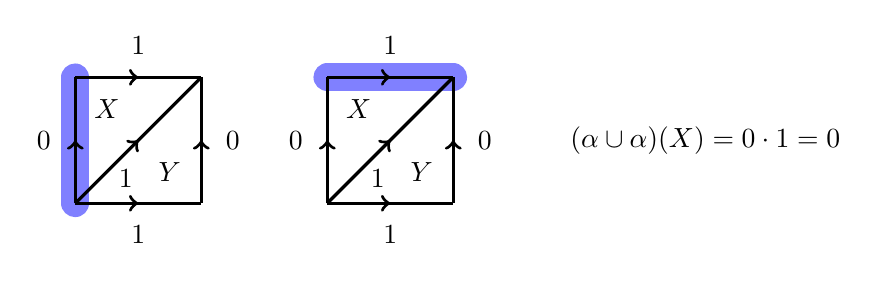
\begin{tikzpicture}[auto,semithick, scale=0.8]
    % a _ a (X)
    \begin{scope}[scale=1,xshift=0cm,very thick]
      \draw[white!50!blue, line width=10pt, line cap=round] (0,0) -- (0,2);
      \begin{scope}[decoration={markings, mark=at position 0.5 with {\arrow{>}}}]
        \draw[postaction={decorate}] (0,0) -- (0,2);
        \draw[postaction={decorate}] (0,0) -- (2,0);
        \draw[postaction={decorate}] (0,2) -- (2,2);
        \draw[postaction={decorate}] (2,0) -- (2,2);
        \draw[postaction={decorate}] (0,0) -- (2,2);
      \end{scope}
      \node (a1) at (1,-0.5)  {$1$};
      \node (a2) at (1,2.5)   {$1$};
      \node (b1) at (-0.5,1)  {$0$};
      \node (b2) at (2.5,1)   {$0$};
      \node (c)  at (0.8,0.4) {$1$};
      \node (X)  at (0.5,1.5) {$X$};
      \node (Y)  at (1.5,0.5) {$Y$};
    \end{scope}
    \begin{scope}[scale=1,xshift=4cm,very thick]
      \draw[white!50!blue, line width=10pt, line cap=round] (0,2) -- (2,2);
      \begin{scope}[decoration={markings, mark=at position 0.5 with {\arrow{>}}}]
        \draw[postaction={decorate}] (0,0) -- (0,2);
        \draw[postaction={decorate}] (0,0) -- (2,0);
        \draw[postaction={decorate}] (0,2) -- (2,2);
        \draw[postaction={decorate}] (2,0) -- (2,2);
        \draw[postaction={decorate}] (0,0) -- (2,2);
      \end{scope}
      \node (a1) at (1,-0.5) {$1$};
      \node (a2) at (1,2.5) {$1$};
      \node (b1) at (-0.5,1) {$0$};
      \node (b2) at (2.5,1) {$0$};
      \node (c)  at (0.8,0.4) {$1$};
      \node (X)  at (0.5,1.5) {$X$};
      \node (Y)  at (1.5,0.5) {$Y$};
    \end{scope}
    \node (m) at (10,1) {$(\alpha \cup \alpha) (X) = 0 \cdot 1 = 0$};
  \end{tikzpicture}
\end{equation*}
\[
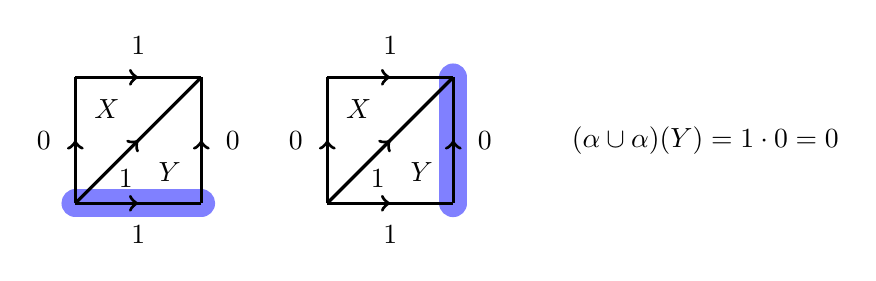
\begin{tikzpicture}[auto,semithick, scale=0.8]
  % a _ a (Y)
  \begin{scope}[scale=1,xshift=0cm,very thick]
    \draw[white!50!blue, line width=10pt, line cap=round] (0,0) -- (2,0);
    \begin{scope}[decoration={markings, mark=at position 0.5 with {\arrow{>}}}]
      \draw[postaction={decorate}] (0,0) -- (0,2);
      \draw[postaction={decorate}] (0,0) -- (2,0);
      \draw[postaction={decorate}] (0,2) -- (2,2);
      \draw[postaction={decorate}] (2,0) -- (2,2);
      \draw[postaction={decorate}] (0,0) -- (2,2);
    \end{scope}
    \node (a1) at (1,-0.5) {$1$};
    \node (a2) at (1,2.5) {$1$};
    \node (b1) at (-0.5,1) {$0$};
    \node (b2) at (2.5,1) {$0$};
    \node (c)  at (0.8,0.4) {$1$};
    \node (X)  at (0.5,1.5) {$X$};
    \node (Y)  at (1.5,0.5) {$Y$};
  \end{scope}
  \begin{scope}[scale=1,xshift=4cm,very thick]
    \draw[white!50!blue, line width=10pt, line cap=round] (2,0) -- (2,2);
    \begin{scope}[decoration={markings, mark=at position 0.5 with {\arrow{>}}}]
      \draw[postaction={decorate}] (0,0) -- (0,2);
      \draw[postaction={decorate}] (0,0) -- (2,0);
      \draw[postaction={decorate}] (0,2) -- (2,2);
      \draw[postaction={decorate}] (2,0) -- (2,2);
      \draw[postaction={decorate}] (0,0) -- (2,2);
    \end{scope}
    \node (a1) at (1,-0.5) {$1$};
    \node (a2) at (1,2.5) {$1$};
    \node (b1) at (-0.5,1) {$0$};
    \node (b2) at (2.5,1) {$0$};
    \node (c)  at (0.8,0.4) {$1$};
    \node (X)  at (0.5,1.5) {$X$};
    \node (Y)  at (1.5,0.5) {$Y$};
  \end{scope}
  \node (m) at (10,1) {$(\alpha \cup \alpha) (Y) = 1 \cdot 0 = 0$};
\end{tikzpicture}
\]


Since $(\alpha \cup \alpha) (X) = 0 = (\alpha \cup \alpha)(Y)$, $\alpha \cup \alpha \in C^2(T;Z)$ is the zero-map. Hence $\alpha \cup \alpha \in H^2(T;Z)$ is zero too.

Earlier we computed $(\alpha \cup \beta) (X) = 0$ and $(\alpha \cup \beta) (Y) = 1$, so $\alpha \cup \beta$ is the map in $C^2(T;Z)$ given by $\{ X \mapsto 0, \; Y \mapsto 1 \}$.

The corresponding map in $H^2(T;Z)$ is the generator $\gamma$ from earlier, so $\alpha \cup \beta = \gamma$.

We could do a similar calculation with diagrams to show that $\beta \cup \beta = 0$ and $\beta \cup \alpha = - \alpha \cup \beta$, but there is a better way.

\begin{theorem}
  For $\alpha \in H^a(X;R)$, $\beta \in H^b(X;R)$, $\alpha \cup \beta = (-1)^{ab}(\beta \cup \alpha)$.
\end{theorem}

This theorem can also be found in Hatcher's \emph{Algebraic Topology} (Theorem 3.11), and actually takes a bit of work to prove. It's worth it though, as it is very useful for cup product calculations. Since $\beta \in H^1(T;Z)$, the theorem implies that $\beta \cup \beta = - \beta \cup \beta$. Since $H^1(T;Z) \cong Z$, the only way this can happen is if $\beta \cup \beta = 0$. This argument works in general: for any $x \in H^k(X;Z)$ with $k$ odd, the theorem implies that $x \cup x = 0$. We demonstrated this above when we calculated $\alpha \cup \alpha = 0$.


We have completed all of the necessary cup product calculations. In summary, $H^*(T;Z)$ is generated by $\alpha$ and $\beta$, which satisfy $\alpha^2 = \beta^2 = 0$ and $\alpha \beta = -\beta \alpha$. (Here when we write $xy$ we mean $x \cup y$.) This means the cohomology is a exterior algebra on two generators with degree 1: $H^*(T;Z) \cong \Lambda_Z(\alpha_1, \beta_1)$.

This is the same result we obtained earlier via the K\"unneth theorem. While the calculation this time was significantly longer and much more involved, it is now clear what exactly these cup products are in terms of cochain maps, and why relations like $\alpha^2 = 0$ hold.

\end{document}


